\section{Инструментарий}

\subsection{Система контроля версий Git}

Для разработки программного комплекса для проведения соревнований в области информационной безопасности было решено использовать Git.\par

Git --- распределённая система управления версиями файлов. Проект был создан Линусом Торвальдсом для управления разработкой ядра Linux  как противоположность  системе управления версиями Subversion (также известная как «SVN»).\par

При работе над одним проектом команде разработчикоа необходим инструмент для совместного написания, резервного копирования и тестирования программного обеспечения. Используя Git, мы имеем:
\begin{itemize}
\item возможность удаленной работы с исходными кодами;
\item возможность создавать свои ветки, не мешая при этом другим разработчикам;
\item доступ к последним изменениям в коде, т.к. все исходники хранятся на сервере git.keva.su;
\item исходные коды защищены, доступ к ним можно получить лишь имея RSA-ключ;
\item возможность откатиться к любой стабильной стадии проекта.
\end{itemize}

Основные постулаты работы с кодом в системе Git:

\begin{itemize}
\item каждая задача решается в своей ветке;
\item необходимо делать коммит как только был получен осмысленный результат;
\item ветка master мержится не разработчиком, а вторым человеком, который производит вычитку и тестирование изменения;
\item все коммиты должны быть осмысленно подписаны/прокомментированы.
\end{itemize}

Для работы над проектом был поднят собственный репозиторий на сервере. Исходные файлы проекта: 
git@gitlab2.keva.su:sibirctf/sibirctf-attack-defense.git\\

\subsection{Система компьютерной вёрстки \LaTeX}

\TeX\ --- это созданная американским математиком и программистом Дональдом Кнутом система для вёрстки текстов. Сам по себе \TeX\ представляет собой специализированный язык программирования.Каждая издательская система представляет собой пакет макроопределений этого языка.\par

\LaTeX\ --- это созданная Лэсли Лэмпортом издательская система на базе \TeX\ 'а.\par 
\LaTeX\ позволяет пользователю сконцентрировать свои услия на содержании и структуре текста, не заботясь о деталях его оформления.\par

Для подготовки отчётной и иной документации нами был выбран \LaTeX\, так как совместно с системой контроля версий Git он предоставляет возможность совместного создания и редактирования документов. Огромным достоинством системы \LaTeX\ то, что создаваемые с её помощью файлы обладают высокой степенью переносимости.\par

Совместно с \LaTeX\ часто используется Bib\TeX\ --- программное обеспечение для создания форматированных списков библиографии. Оно входит в состав дистрибутива \LaTeX\ и позволяет создавать удобную, универсальную и долговечную библиографию. Bib\TeX\ стал одной из причин, по которой нами был выбран \LaTeX\ для создания документации.\\

\subsection{Система мониторинга сервисов компьютерной сети Zabbix}

Zabbix ---  свободная система мониторинга и отслеживания статусов разнообразных сервисов компьютерной сети, серверов и сетевого оборудования. \par

Архитектура Zabbix:
\begin{itemize}
\item Zabbix-сервер — это ядро программного обеспечения Zabbix. Сервер может удаленно проверять сетевые сервисы, является хранилищем, в котором находятся все конфигурационные, статистические и оперативные данные;
\item Zabbix-прокси — собирает данные о производительности и доступности от имени Zabbix сервера. Все собранные данные заносятся в буфер на локальном уровне и передаются Zabbix серверу, к которому принадлежит прокси-сервер;
\item Zabbix-агент — контроль локальных ресурсов и приложений (таких как жесткие диски, память, статистика процессора и т. д.) на сетевых системах. Эти системы должны работать с запущенным Zabbix агентом;
\item Веб-интерфейс — интерфейс является частью Zabbix сервера, и, как правило (но не обязательно), запущен на том же физическом сервере, что и Zabbix сервер. Работает на PHP, требует веб-сервер (например, Apache).
\end{itemize}

\begin{figure}[h!]
    \centering
    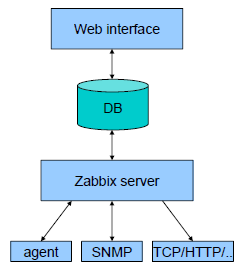
\includegraphics[width=0.38\textwidth]{zabbix}
    \caption{Система мониторинга Zabbix}
    \label{img:0}
\end{figure} 

\subsection{Язык программирования Python}

Python --- высокоуровневый язык программирования общего назначения, ориентированный на повышение производительности разработчика и читаемости кода. Синтаксис ядра Python минималистичен. В то же время стандартная библиотека включает большой объём полезных функций. \par

Основные архитектурные черты — динамическая типизация, автоматическое управление памятью, полная интроспекция, механизм обработки исключений, поддержка многопоточных вычислений и удобные высокоуровневые структуры данных. Код в Python организовывается в функции и классы, которые могут объединяться в модули.\par

Основными преимуществами языка программирования Python являются большое количество библиотек, кроссплатформенность, широкие возможности профилирования кода. \par

Язык обладает чётким и последовательным синтаксисом, продуманной модульностью и масштабируемостью, благодаря чему исходный код написанных на Python программ легко читаем. При передаче аргументов в функции Python использует вызов по соиспользованию.\par

Разработка языка Python была начата в конце 1980-х годов сотрудником голландского института CWI Гвидо ван Россумом.\\

\subsection{Система управления проектами и задачами Teamwork}

Teamwork --- это сервис, предоставляющий возможность управлять своими проектами, задачами, персоналом.\par

Основным преимуществом является удобный интерфейс управления проектом, этапами (вехами), задачами. \par
Проект можно разбить на списки отдельных задач, привязывая их к определенным этапам, а также ограничивая определенным кругом лиц. \par
Каждой задаче можно назначить одного и более ответственного, установить приоритет, назначить дату начала и окончания, добавить описание, а также настроить оповещение в случае наступления срока окончания задачи.\par

Программа бесплатна при условии, что команда работает только над одним проектом.\par

Также доступна диаграмма Ганта.\\

\clearpage